\section{ADVENT NOPELE OLANSI DAMIAHAN SIHITE (1174089)}
\subsection{Menulis Shapefile dengan PySHP}
\begin{enumerate}
	\item Nomor 1
	\lstinputlisting{src/tugas2/1174089/1.py}
	\begin{figure}[H]
		
\includegraphics[width=6cm]{figures/Tugas2/1174089/1.PNG}
		\centering
		\caption{Point (Titik)}
	\end{figure}
	\item Nomor 2
	\lstinputlisting{src/tugas2/1174089/2.py}
	\begin{figure}[H]
		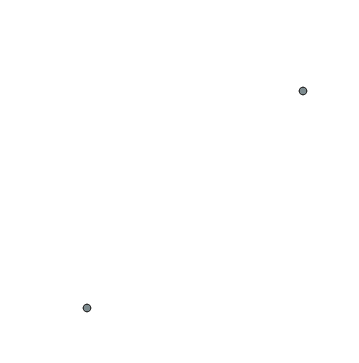
\includegraphics[width=6cm]{figures/Tugas2/1174089/2.PNG}
		\centering
		\caption{Point (Titik)}
	\end{figure}
	\item Nomor 3
	\lstinputlisting{src/tugas2/1174089/3.py}
	\begin{figure}[H]
		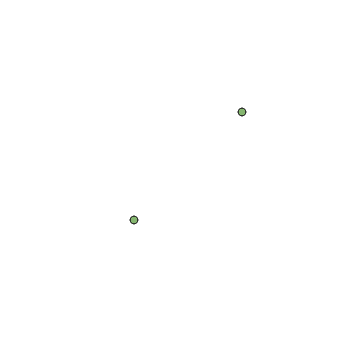
\includegraphics[width=6cm]{figures/Tugas2/1174089/3.PNG}
		\centering
		\caption{Point (Titik)}
	\end{figure}
	\item Nomor 4
	\lstinputlisting{src/tugas2/1174089/4.py}
	\begin{figure}[H]
		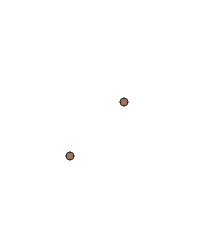
\includegraphics[width=6cm]{figures/Tugas2/1174089/4.PNG}
		\centering
		\caption{Point (Titik)}
	\end{figure}
	\item Nomor 5
	\lstinputlisting{src/tugas2/1174089/5.py}
	\begin{figure}[H]
		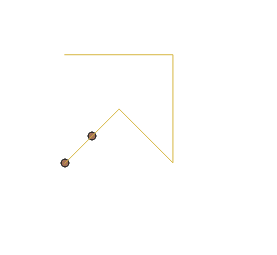
\includegraphics[width=6cm]{figures/Tugas2/1174089/5.PNG}
		\centering
		\caption{PolyLine (Garis)}
	\end{figure}
	\item Nomor 6
	\lstinputlisting{src/tugas2/1174089/6.py}
	\begin{figure}[H]
		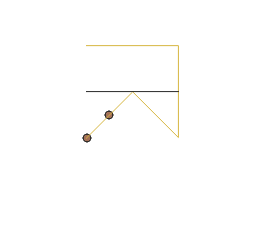
\includegraphics[width=6cm]{figures/Tugas2/1174089/6.PNG}
		\centering
		\caption{Polygon (Bidang)}
	\end{figure}
	\item Nomor 7
	\lstinputlisting{src/tugas2/1174089/7.py}
	\begin{figure}[H]
		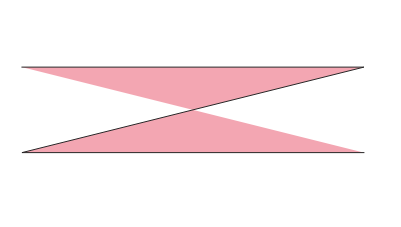
\includegraphics[width=6cm]{figures/Tugas2/1174089/7.PNG}
		\centering
		\caption{Polygon (Bidang)}
	\end{figure}
	\item Nomor 8
	\lstinputlisting{src/tugas2/1174089/8.py}
	\begin{figure}[H]
		
\includegraphics[width=6cm]{figures/Tugas2/1174089/8.PNG}
		\centering
		\caption{Polygon (Bidang)}
	\end{figure}
	\item Nomor 9
	\lstinputlisting{src/tugas2/1174089/9.py}
	\begin{figure}[H]
		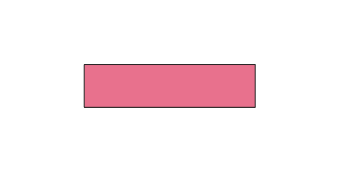
\includegraphics[width=6cm]{figures/Tugas2/1174089/9.PNG}
		\centering
		\caption{Polygon (Bidang)}
	\end{figure}
	\item Nomor 10
	\lstinputlisting{src/tugas2/1174089/10.py}
	\begin{figure}[H]
		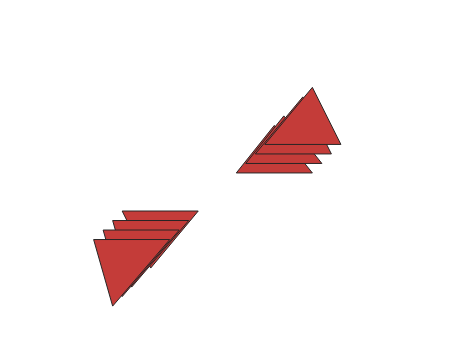
\includegraphics[width=6cm]{figures/Tugas2/1174089/10.PNG}
		\centering
		\caption{Polygon, Hasil modulus dari npm saya 1174089 adalah  membuatsegitiga sama sisi dan angka akhir dari npm saya adalah 8 jadi membuat bidangnya sebanyak 8}
	\end{figure}
\end{enumerate}
\subsection{Link}
https://youtu.be/KCN3zfrJMbs